\section{Detecting Anomalous Transactions using KDE}

\subsection{Designing a custom KDE Class}

The KDE class with the Epachnikov kernel

\begin{equation}
    K(x) = \frac{3}{\pi} (1 - ||x||_2^2) \quad \text{if} \quad ||x||_2 \leq 1
\end{equation}

The code was implemented in the file \texttt{2.py}.

\subsection{Estimating Distribution of Transactions}

After estimating the distribution of transactions using the Epachnikov kernel, the estimated probability density graph is shown in Figure \ref{fig:q2_1}.

\begin{figure}[H]
    \centering
    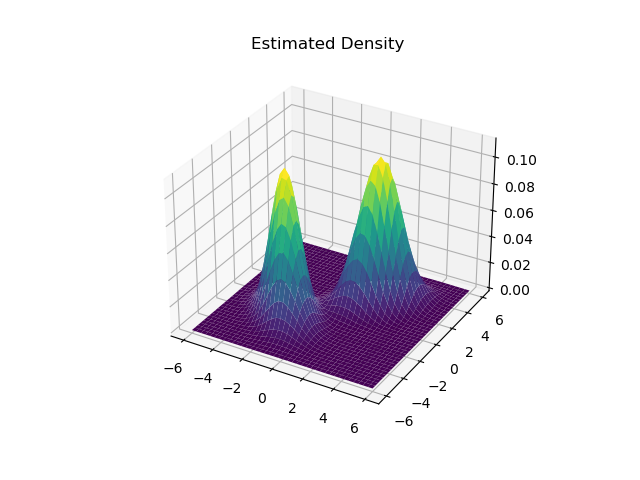
\includegraphics[width=0.8\textwidth]{../q2/images/transaction_distribution.png}
    \caption{Estimated Probability Density of Transactions}
    \label{fig:q2_1}
\end{figure}

\newpage